% !TEX root = ../main.tex
%-------------------------------------------------------------------------------
%-------------------------------------------------------------------------------
\begin{frame}\begin{center}
		\LARGE\textit{Economic model}
\end{center}\end{frame}
%-------------------------------------------------------------------------------
%-------------------------------------------------------------------------------
\begin{frame}
\textbf{Decision Problem}
\begin{align*}\begin{array}{ll}
t = 1, \hdots, T& \text{decision period} \\
s\in S & \text{state}  \\
a\in A & \text{action} \\
d_t(s) & \text{decision rule} \\
r_t(s, a) & \text{immediate reward}\\
\end{array}\end{align*}
\end{frame}
%-------------------------------------------------------------------------------
%-------------------------------------------------------------------------------
\begin{frame}
\begin{center}\textbf{Timing of Events}\vspace{0.9cm}
\scalebox{0.9}{\hspace{-0.2cm}%!TEX root = ../main.tex

\definecolor{light-gray}{gray}{0.85}


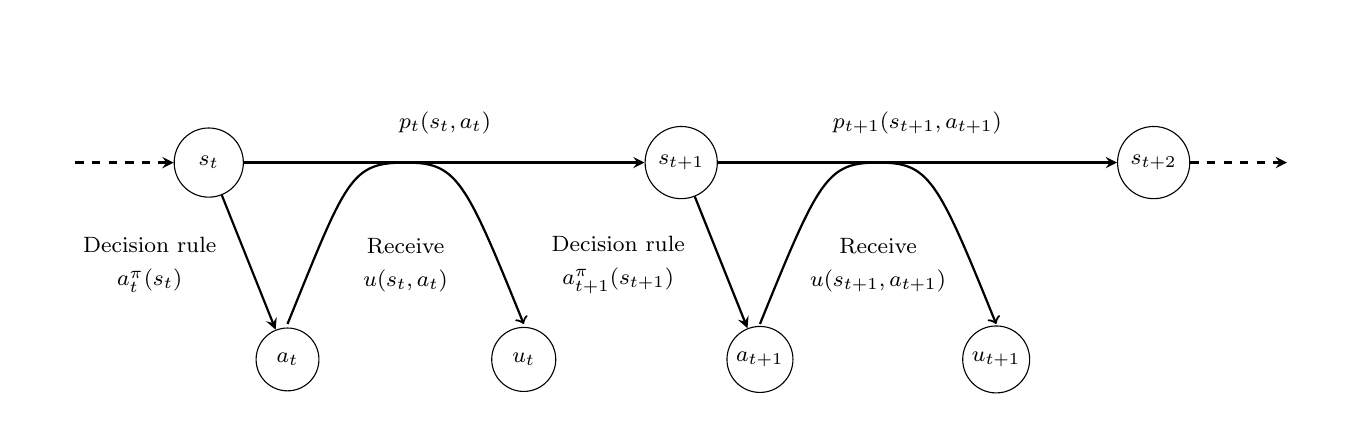
\begin{tikzpicture}[node distance=2cm]
%define styles
\tikzstyle{startstop} = [circle, rounded corners, minimum width=0.6cm, minimum height=0.3cm,text centered, draw=black]
[
->,
>=stealth',
auto,node distance=3cm,
thick,
main node/.style={circle, draw, font=\sffamily\Large\bfseries}
]
\tikzstyle{arrow} = [thick,->,>=stealth]]
\tikzstyle{darrow} = [dotted,->,>=stealth]]
%first and second column

\node (r0) [startstop, xshift = -3cm, draw = none] {}; 
\node (r999) [startstop, xshift = 13cm, draw = none] {}; 

\node (r1) [startstop, xshift = -1cm] {\footnotesize $~\,s_t\,~$};
\node (r2) [startstop, xshift = 5cm] {\footnotesize $s_{t+1}$};  %previously 4
\node (r3) [startstop, xshift = 11cm] {\footnotesize $s_{t+2}$}; %previously 8

\draw [arrow, dashed] (r0) -- node[anchor=south] {} (r1) ;
\draw [arrow] (r1) -- node[anchor=south] {} (r2) ;
\draw [arrow] (r2) -- node[anchor=south] {} (r3) ;
\draw [arrow, dashed] (r3) -- node[anchor=south] {} (r999) ;

\node (r4) [startstop, xshift = 0 cm, yshift = -2.5cm, inner sep = 0.08cm] {\footnotesize $~\,a_t\,~$ };
\node (r5) [startstop, xshift = 3 cm, yshift = -2.5cm, inner sep = 0.08cm] {\footnotesize $~\,u_t\,~$ };
\node (r6) [startstop, xshift = 6 cm, yshift = -2.5cm, inner sep = 0.08cm] {\footnotesize $a_{t+1}$ };
\node (r7) [startstop, xshift = 9 cm, yshift = -2.5cm, inner sep = 0.08cm] {\footnotesize $u_{t+1}$ };

\draw [arrow] (r1) -- node[anchor=south] {} (r4) ;
\draw [arrow] (r2) -- node[anchor=south] {} (r6) ;

\draw[ thick](0,-2.05).. controls (0.75, -0.2) and (0.8,0)..(1.5, 0);
\draw[->, thick](1.5, 0).. controls (2.15, 0) and (2.25, -0.2)..(3, -2.05);
\draw[ thick](6,-2.05).. controls (6.75, -0.2) and (6.85,0)..(7.5, 0);
\draw[->, thick](7.5, 0).. controls (8.15, 0) and (8.25,-0.2)..(9, -2.05);

\node(r8)[startstop, xshift = - 1.75cm, yshift = -1.3cm, draw =none, align=center] {\footnotesize Decision rule \\ \footnotesize $a_t^{\pi}(s_t)$ };
\node(r9)[startstop, xshift= 4.2cm, yshift = -1.3cm, draw =none, align = center] {\footnotesize Decision rule \\ \footnotesize $a_{t+1}^{\pi}(s_{t+1})$ };
%\node(r10)[startstop, yshift = 1cm, xshift = 2cm, draw =none, align=center ] {\footnotesize Transition probability\\ \footnotesize distribution \\ \footnotesize $p_t(s_t, a_t)$};
%\node(r11)[startstop, yshift = 1cm, xshift = 8cm, draw =none, align=center ] { \footnotesize Transition probability\\ \footnotesize distribution \\ \footnotesize $p_{t+1}(s_{t+1}, a_{t+1})$};
\node(r10)[startstop, yshift = 0.5cm, xshift = 2cm, draw =none, align=center ] {\footnotesize $p_t(s_t, a_t)$};
\node(r11)[startstop, yshift = 0.5cm, xshift = 8cm, draw =none, align=center ] {\footnotesize $p_{t+1}(s_{t+1}, a_{t+1})$};
\node(r12)[startstop, yshift = -1.3cm, xshift = 1.5cm, draw =none, align=center ] {\footnotesize Receive\\ \footnotesize  $u(s_t, a_t)$ };
\node(r13)[startstop, yshift = -1.3cm, xshift = 7.5cm, draw =none, align=center ] {\footnotesize Receive\\ \footnotesize  $u(s_{t+1}, a_{t+1})$ };

\end{tikzpicture}


% OLd figure timing of events
%
%	\begin{tikzpicture}[scale=1.0, every node/.style={scale=0.8}]
%
%	\tikzset{
%	eqblock/.style={text width=3.5cm,align=center}
%	}
%
%	% Nodes
%	\node[xshift=-6cm] (left) {};
%	\node[below=3cm of left, xshift=6cm] (bottom_left) {};
%	\node[node distance=6cm, right of=left, xshift=6cm] (right) {};
%	\node[node distance=6cm, right of=bottom_left, xshift=6cm] (bottom_right) {};
%
%	\node[node distance=6cm, right of=left, yshift=-.5cm] (t1) {\large$t$};
%	\node[node distance=6cm, right of=bottom_left, yshift=-.5cm] (t2) {\large$t+1$};
%
%	\node[eqblock, above of=left, xshift=3cm] (eq1) {\large$\{u(s_t, a_t)\}_{a_t\in A}$};
%	\node[eqblock, above of=left, xshift=6cm] (eq2) {\large$a_t$};
%	\node[eqblock, above of=left, xshift=9cm] (eq3) {\large$u(s_t, a_t)$};
%	\node[eqblock, above of=bottom_left, xshift=2cm] (eq4) {\large$\{u(s_{t + 1}, a_{t + 1}\noindent )\}_{a_{t + 1}\in A}$};
%	\node[eqblock, above of=bottom_left, xshift=6cm] (eq6) {\large$a_{t + 1}$};
%	\node[eqblock, above of=bottom_left, xshift=9cm] (eq5) {\large$u(s_{t + 1}, a_{t + 1})$};
%
%	\node[above of=eq1, node distance=1cm] (text2) {\large Learn};
%	\node[above of=eq2, node distance=1cm] (text3) {\large Choose};
%	\node[above of=eq3, node distance=1cm] (text1) {\large Receive};
%	\node[above of=eq4, node distance=1cm] (text4) {\large Learn};
%	\node[above of=eq6, node distance=1cm] (text5) {\large Choose};
%	\node[above of=eq5, node distance=1cm] (text6) {\large Receive};
%
%	% Lines
%	\draw[|-|] (left) -- (right);
%	\draw[|-|] (bottom_left.center) -- (bottom_right);
%
%	\end{tikzpicture}

}
\end{center}
\end{frame}
%-------------------------------------------------------------------------------
%-------------------------------------------------------------------------------
\begin{frame}
\begin{align*}\begin{array}{ll}
\pi = (d_1, \hdots, d_T) & \text{policy}\\
\delta & \text{discount factor} \\
p_t(s, a) & \text{conditional distribution}
\end{array}\end{align*}
\end{frame}
%-------------------------------------------------------------------------------
%-------------------------------------------------------------------------------
\begin{frame}
\textbf{Individual's Objective under Risk}\vspace{0.3cm}
\begin{align*}
v^{\pi^*}_1(s) = \max_{\pi\in\Pi} \E_{s}^\pi\left[\sum^{T}_{t = 1}  \delta^{t - 1} r_t(X_t, d_t(X_t))\right]
\end{align*}
\end{frame}
%-------------------------------------------------------------------------------
%-------------------------------------------------------------------------------
